% flatex input: [lambda_1_lambda_2.tex]

\begin{figure}[h]
\centering
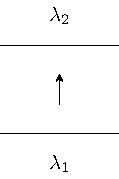
\includegraphics{fig_lambda_1_lambda_2.pdf}
\caption{Partition function between two boundary states $\lambda_1$ and $\lambda_2$}
\label{Fig in lambda_1_lambda_2}
\end{figure}

In this appendix, we will generalize the calculation in App.~\ref{app:gnd_dn_lambda} to boundary states specified by $\lambda_1$ and $\lambda_2$. In particular we would like to calculate the amplitude for the setup shown in Fig.~\ref{Fig in lambda_1_lambda_2}, using the boundary state approach as in App.~\ref{app:gnd_dn_lambda}. With the same notation, the partition function reads
\begin{equation}
Z_{ab} = \langle 0 | \exp\Big\{ \vec{b} R_a^* \vec{\bar{b}}\Big\} \exp\Big\{ - \vec{b}^{\dagger} \mathbb{I}_2 \otimes M  \vec{b} \Big\}   \exp\Big\{  \vec{b}^{\dagger} R_b  \vec{\bar{b}}^{\dagger}\Big\}  |0  \rangle  = \frac{1}{\det ( 1 - R^{\dagger} _a  e^{- \mathbb{I}_2 \otimes M} R_b) }
\end{equation}
where
\begin{equation}
M =  \frac{4\pi^2}{\beta} \text{diag}( 1, 2, \cdots )
\end{equation}
and $R_a$($R_b$) correspond to the $\lambda_1$($\lambda_2$) boundary conditions. Using the fact that their determinants are $\det( R_a R_b^{\dagger})  = 1$, we have
\begin{equation}
\begin{aligned}
F &= - \ln Z_{ab} = \ln \det ( R_a R_b^{\dagger} - e^{- \mathbb{I}_2 \otimes M} )\\
& = \ln \det 
\begin{bmatrix}
\cos 2 \Delta \theta \mathbb{I} - e^{-M}   & \sin 2 \Delta \theta \mathbb{I}\\
- \sin 2\Delta \theta \mathbb{I}  &   \cos 2 \Delta \theta \mathbb{I} - e^{-M} \\ 
\end{bmatrix} \\
& = \sum_i \ln [ 1 - 2 \cos 2 \Delta \theta e^{- \lambda_i } + e^{- 2 \lambda_i }  ] \\
& = \frac{\beta}{4\pi^2} \int_0^{\infty} dx \ln [ 1 - 2 \cos 2 \Delta \theta e^{-x} + e^{-2x} ] 
\end{aligned}
\end{equation}
where $\Delta \theta = \theta_2 - \theta_1$. This integral is an even function of $\Delta \theta$ and the $\Delta \theta > 0$ case reduce to the polylog and Bernoulli polynomial
\begin{equation}
\begin{aligned}
  F &= \frac{\beta}{4\pi^2} \left[ - \text{Li}_2 ( e^{2i |\Delta \theta|} ) - \text{Li}_2 ( e^{- 2i |\Delta \theta|} ) \right] \\
  & = \frac{\beta}{4\pi^2}  \left[ - 2\pi^2 B_2 (x) \right] \\
  &= - \frac{\beta}{2} B_2( |x| ) 
\end{aligned}
\end{equation}
where $x = \frac{\Delta \theta}{ \pi}$. 
